% -*- root: ../thesis.tex -*- 

\chapter[Programming with actors in Java 8]{Programming with actors in Java~8%
\footnote{This paper is funded by the EU project FP7-610582 ENVISAGE: Engineering Virtualized Services, \surl{http://www.envisage-project.eu}.}
}
% 
\label{ch:p02:ch01}
% 
\chapterauthor{Behrooz Nobakht, Frank S. de Boer}

\section*{Abstract}
There exist numerous languages and frameworks that support an implementation of a variety of actor-based programming models in Java using concurrency utilities and threads.
% 
Java~8 is released with fundamental new features: lambda expressions and further dynamic invocation support.
%
We show in this paper that such features in Java~8 allow for a high-level actor-based methodology for programming distributed systems which supports the programming to interfaces discipline.
%
The embedding of our actor-based Java API is shallow in the sense that it abstracts from the actual thread-based deployment models. 
%
We further discuss different concurrent execution and thread-based deployment models and an extension of the API for its actual parallel 
and distributed implementation.
% 
We present briefly the results of a set of experiments which provide evidence of  the potential impact of lambda expressions in Java~8  regarding the adoption of the actor concurrency model in large-scale distributed applications.

% 

\subparagraph*{Conference Publication}
\emph{Lecture Notes in Computer Science, Volume 8803, 6th International Symposium on Leveraging Applications of Formal Methods, Verification and Validation with Specialized Techniques and Applications -- ISoLA 2014, Pages 37--53, DOI 
\smalltt{10.1007/978-3-662-45231-8\_4}}

% 

% \keywords{Actor model, Concurrency, Asynchronous Message, Java, Lambda Expression}

\section{Introduction}
\label{ch03:sec:introduction}
Java is beyond doubt one of the mainstream object oriented programming languages 
that supports a \emph{programming to interfaces} discipline \cite{oop:patterns,oop:survey}.
Through the years, Java has evolved from a mere programming language to a huge platform to drive and envision standards for mission-critical business applications.
Moreover, the Java language itself has evolved in these years to support its community with new language features and standards.
One of the noticeable domains of focus in the past decade has been distribution and concurrency in research and application.
This has led to valuable research results and numerous libraries and frameworks with an attempt to provide distribution and concurrency at the level of Java language.
However, it is widely recognized that the thread-based model of concurrency in Java that is a well-known approach is not appropriate for realizing distributed systems because of its inherent synchronous communication model.
On the other hand, the event-driven actor model of concurrency introduced by Hewitt \cite{Hewitt69} is 
a powerful concept for modeling distributed and concurrent
systems \cite{Agha90,agha97}. 
Different extensions of actors are proposed in several domains and are claimed to be the most suitable model of computation for many  applications \cite{Hewitt07-commitment}. 
Examples of these domains include designing embedded systems \cite{LeeACtorEmbedded03,LeeLN09}, 
wireless sensor networks \cite{CheongSensor05}, multi-core programming \cite{KarmaniSA09} 
and delivering cloud services through SaaS or PaaS \cite{Chang:DAIS07}.
This model of concurrent computation forms the basis of the
programming languages Erlang \cite{Armstrong10Erlang} and Scala
\cite{haller09tcs} that have recently gained in popularity, in part
due to their support for scalable concurrency.  Moreover, based on the
Java language itself, there are numerous libraries  that
provide  an implementation of an actor-based programming model.  

% The main problem addressed in this paper is that in general existing actor-based programming techniques use extension and inheritance over composition of interfaces; 
% i.e. they require explicit inheritance of objects to allow for message passing and handling through specific methods designed in the framework or technique.
% They allow for generic and efficient invocation of special methods in objects that handle messages by inheritance.
% However, they \emph{bypass} the the basis of programming to interfaces and design-by-contract discipline~\cite{meyer:design}.
% This style of combination of object orientation and event-driven (or asynchronous messaging) in such frameworks and techniques makes actor-based programs developed difficult to reason about and formalize.
% This clearly hampers the promotion of actor-based programming in mainstream industry which is heavily based on object-oriented software engineering practice.
% 
% The main result of this paper is a Java API for programming distributed systems
% using asynchronous message passing and a corresponding actor-based programming methodology 
% which abstracts invocation from execution (e.g. thread-based deployment).
% The Java API fundamentally follows programming to interfaces discipline such that implementations only utilize a natural object-oriented design approach to program with actors.
% The API is desgined and implemented using Java~8 features.
% We further discuss the API architecture, its properties, and different concurrent execution models for the actual implementation.
% 
% Our main approach consists of the explicit realization of an actor in terms of its \emph{interface}.
% To this goal, a set of features including lambda expressions introduced in Java~8 are used in the  implmentation of asynchronous message passing and actor model.
% The corresponding actor-based methodology is formalized in terms of an executable modelling language
% which lends itself to formal analysis and verification, ABS~\cite{johnsen2012abs}.
% We provide a semantic translation of the concurrent modelling language ABS into Java~8.
% We present the operational semantics of such translation and how model extraction is a direct benefit of an implementation based on such API.

The main problem addressed in this paper is that in general existing actor-based programming techniques
are based on an explicit encoding of mechanisms at the application level for message passing and handling, 
and as such overwrite the general object-oriented approach of method look-ups that 
forms the basis of programming to interfaces and the design-by-contract discipline~\cite{meyer:design}.
The entanglement of event-driven (or asynchronous messaging) and object-oriented method look-up 
makes  actor-based programs developed using such techniques extremely difficult to  reason about and formalize.
This clearly hampers the promotion of actor-based programming in mainstream industry that heavily practices object-oriented software engineering.

The main result of this paper is a Java~8 API for programming distributed systems
using asynchronous message passing and a corresponding actor programming methodology 
which abstracts invocation from execution (e.g. thread-based deployment) and fully supports
 programming to interfaces discipline.
We  discuss the API architecture, its properties, and different concurrent execution models for the actual implementation.

Our main approach consists of the explicit description of an actor in terms of its \emph{interface}, 
the use of the recently introduced lambda expressions in Java~8 in the  implementation of asynchronous message passing,  
and the formalization of a corresponding high-level actor programming methodology in terms of an executable modeling language
which lends itself to formal analysis, ABS ~\cite{johnsen2012abs}.
% We provide a semantic translation of the concurrent modelling language ABS~\cite{johnsen2012abs} into Java~8 supporting actor programming.
% We present the operational semantics of such translation and how model extraction be a direct benefit of an implementation based on such API.

The paper continues as follows: 
in Section \ref{ch03:sec:relatedwork}, we briefly discuss a set of related works on actors and concurrent models especially on JVM platform. 
Section \ref{ch03:sec:example} presents an example that we use throughout the paper, we start to model the example using a library. 
Section \ref{ch03:sec:actor:programming} briefly introduces a concurrent modeling language and implements the example.
Section \ref{ch03:sec:j8:features} briefly discusses Java 8 features that this works uses for implementation.
Section \ref{ch03:sec:j8:actors:realization} presents how an actor model maps into programming in Java~8.
Section \ref{ch03:sec:impl:arch} discusses in detail the implementation architecture of the actor API.
Section \ref{ch03:sec:experiments} discusses how a number of benchmarks were performed for the implementation of the API and how they compare with current related works.
Section \ref{ch03:sec:conclusion} concludes the paper and discusses the future work.

 
\section{Related Work}
\label{ch03:sec:relatedwork}

There are numerous works of research and development in the domain of actor modeling and implementation in different languages.
We discuss a subset of the related work in the level of modeling and implementation with more focus on Java and JVM-based efforts in this section.

Erlang \cite{Armstrong10Erlang} is a programming language used to build massively scalable soft real-time systems with requirements on high availability. 
Some of its uses are in telecoms, banking, e-commerce, computer telephony and instant messaging. Erlang's runtime system has built-in support for concurrency, distribution and fault tolerance.
While threads require external library support in most languages, Erlang provides language-level features for creating and managing processes with the aim of simplifying concurrent programming. 
Though all concurrency is explicit in Erlang, processes communicate using message passing instead of shared variables, which removes the need for locks.
Elixir \cite{elixir} is a functional meta-programming aware language built on top of the Erlang VM. It is a dynamic language with flexible syntax with macros support that leverages Erlang's abilities to build concurrent, distributed, fault-tolerant applications with hot code upgrades.

Scala is a hybrid object-oriented and functional programming language inspired by Java. 
The most important concept introduced in \cite{haller09tcs} is that Scala actors unify
\textit{thread-based} and \textit{event-based} programming model to fill the gap for concurrency programming. 
Through the event-based model, Scala also provides the notion of continuations. 
Scala provides quite the same features of scheduling of tasks as in concurrent Java; 
i.e., it does not provide a direct and customizable platform to manage and schedule priorities on messages sent to other actors.
Akka \cite{haller2012integration} is a toolkit and runtime for building highly concurrent, distributed, and fault tolerant event-driven applications on the JVM based on actor model.
% Akka implements a hybrid of the actor model, fault tolerance through a
% ``let it crash'' mind set, and location transparency to support distributed environments.

Kilim \cite{srinivasan2008kilim} is a message-passing framework for Java that provides ultra-lightweight threads and facilities for fast, safe, zero-copy messaging between these threads.
It consists of a bytecode postprocessor (a ``weaver''), a run time library with buffered mailboxes (multi-producer, single consumer queues) and a user-level scheduler and a type system that puts certain constraints on pointer aliasing within messages to ensure interference-freedom between threads.
% 
The SALSA \cite{varela2007salsa,KarmaniSA09} programming language (Simple Actor Language System and Architecture) is an active object-oriented programming language that uses concurrency primitives beyond asynchronous message passing, including token-passing, join, and first-class continuations.
% 
% Clojure \cite{hickey2008clojure} is a dynamic programming language that targets the Java Virtual Machine. 
% It is designed to be a general-purpose language, combining the approachability and interactive development of a scripting language with an efficient and robust infrastructure for multithreaded programming. 
% Clojure is a compiled language - it compiles directly to JVM bytecode, yet remains completely dynamic.
% Clojure is influenced by Scheme \cite{scheme} which is a Lisp dialect.
% Scheme was introduced through ``Lambda Papers''.
 % \footnote{\url{http://en.wikipedia.org/wiki/Lambda\_Papers\#The\_Lambda_Papers}}.
% Neither Clojure nor scheme do directly implement the actor model, however, through functional programming of lambda calculus that they provide, they are suitable for concurrent applications built with lambda statements.

RxJava \cite{rxjava} by Netflix is an implementation of reactive extensions \cite{rx} from Microsoft.  
Reactive extensions try to provide a solution for composing asynchronous and event-based software using observable pattern and scheduling.  
An interesting direction of this library is that it uses reactive programming to avoid a phenomenon known as ``callback hell''; a situation that is a natural consequence of composing \jtt{Future} abstractions in Java specifically when they wait for one another.  
However, RxJava advocates the use of asynchronous functions that are triggered in response to the other functions.
% 
In the same direction, LMAX Disruptor \cite{lmax,lmax:mf} is a highly concurrent event processing framework that takes the approach of event-driven programming towards provision of concurrency and asynchronous event handling.
The system is built on the JVM platform and centers on a Business Logic Processor that can handle 6 million events per second on a single thread. 
The Business Logic Processor runs entirely in-memory using event sourcing. 
The Business Logic Processor is surrounded by Disruptors - a concurrency component that implements a network of queues that operate without needing locks.

\section{State of the Art: An example}
\label{ch03:sec:example}
In the following, we illustrate the state of the art in actor programming by means of a simple example using
the Akka~\cite{akka} library which features asynchronous messaging and which is used to program actors in both Scala and Java.
We want to model in Akka an ``asynchronous ping-pong match'' between two actors represented by the 
two interfaces \jtt{IPing} and \jtt{IPong} which are depicted in Listings \ref{ch03:lst:ping:interface} and \ref{ch03:lst:pong:interface}.
An asynchronous call by the actor implementing the \jtt{IPong} interface of the \jtt{ping} method of the actor
implementing the \jtt{IPing} interface should generate an asynchronous call of the \jtt{pong} method of the callee,
and vice versa.
We intentionally design \jtt{ping} and \jtt{pong} methods to take  arguments in order to demonstrate 
how method arguments may affect the use of an actor model in an object-oriented style.





\lstset{language=Java}
\begin{center}
\begin{minipage}[t]{0.48\textwidth}
\begin{lstlisting}[caption=Ping as an interface,label=ch03:lst:ping:interface]
public interface IPing {
  void ping(String msg);
}
\end{lstlisting}
\end{minipage}
\hfill
\begin{minipage}[t]{0.48\textwidth}
\begin{lstlisting}[caption=Pong as an interface,label=ch03:lst:pong:interface]
public interface IPong {
  void pong(String msg);
}
\end{lstlisting}
\end{minipage}
\end{center}

To model an actor in Akka by a class, say  \jtt{Ping},  with interface \jtt{IPing}, this class is required  \emph{both} to \emph{extend}
a given pre-defined  class \jtt{UntypedActor}  and \emph{implement} the interface \jtt{IPing}, 
as depicted in Listings \ref{ch03:lst:ping:akka} and \ref{ch03:lst:pong:akka}.
The class \jtt{UntypedActor} provides two Akka framework methods \jtt{tell} and \jtt{onReceive} 
which are used to enqueue and dequeue asynchronous messages.
An asynchronous call to, for example,  the method \jtt{ping} then can be modeled by passing a user-defined  encoding of this call,
in this case by prefixing the string argument with the string ``pinged'', to a (synchronous) call
of the \jtt{tell} method which results in enqueuing the message.
In case this message is dequeued
the implementation of the \jtt{onReceive} method as provided by the \jtt{Ping} class then calls the \jtt{ping} method.

\lstset{language=Java}
\begin{center}
\begin{minipage}[t]{0.48\textwidth}
\begin{lstlisting}[caption=Ping actor in Akka,label=ch03:lst:ping:akka]
public class Ping(ActorRef pong)
  extends UntypedActor 
  implements IPing {

  public void ping(String msg) {
    pong.tell("ponged," + msg)
  }

  public void onReceive(Object m) {
    if (!(m instanceof String)) {
      // Message not understood.
    } else 
    if (((String) m).startsWith("pinged") {
      // Explicit cast needed.
      ping((String) m);
    } 
   }
}
\end{lstlisting}
\end{minipage}
\hfill
\begin{minipage}[t]{0.48\textwidth}
\begin{lstlisting}[caption=Pong class in Akka,label=ch03:lst:pong:akka]
public class Pong 
  extends UntypedActor 
  implements IPong {

  public void pong(String msg) {
    sender().tell(
      "pinged," + msg); 
  }

  public void onReceive(Object m) {
    if (!(m instanceof String)) {
      // Message not understood.
    } else 
    if (m.startsWith("ponged") {
      // Explicit cast needed.
      ping((String) m);
    } 
   }
}
 
\end{lstlisting}
\end{minipage}
\end{center}

Access to the sender of the message in Akka is provided by \jtt{sender()}.
In the main method as described in Listing \ref{ch03:lst:main:akka} we show how the initialize and start the ping/pong match.
Note that a reference to the ``pong'' actor is passed to the ``ping'' actor.

\begin{figure}[h]
% \begin{wrapfigure}{r}{0.48\textwidth}
% \vspace{-20pt}
\begin{lstlisting}[caption=main in Akka,label=ch03:lst:main:akka]
ActorSystem s = ActorSystem.create();
ActorRef pong = s.actorOf(Props.create(Pong.class));
ActorRef ping = s.actorOf(Props.create(Ping.class, pong));
ping.tell(""); // To get a Future
\end{lstlisting}
% \vspace{-20pt}
% \end{wrapfigure}
\end{figure}

Further, both the \jtt{onReceive} methods are invoked by Akka \jtt{ActorSystem} itself. 
In general, Akka actors are of type  \jtt{ActorRef} which is an abstraction provided by Akka to allow actors send asynchronous messages to one another.
% 
An immediate consequence  of the above use of inheritance is that the class \jtt{Ping} is now exposing a public behavior 
that is \emph{not} specified by its \emph{interface}. 
Furthermore, a ``ping'' object refers to a ``pong'' object by the type \jtt{ActorRef} .
This means that the interface \jtt{IPong} is not directly visible to the ``ping'' actor.
Additionally, the implementation details of receiving a message should be 
``hand coded'' by the programmer into the  special method \jtt{onReceive} to define the  responses to the received messages.
In our case, this implementation consists of a decoding of the message  (using type-checking)
in order to \emph{look up} the method that subsequently should be invoked.
This fundamentally interferes with the general object-oriented mechanism for method look-up which forms the basis of the programming to interfaces discipline.
In the next section, we continue the same example and discuss an actor API for directly calling asynchronously methods
using the general object-oriented mechanism for method look-up.
Akka has recently released a new version that supports Java 8 features
\footnote{Documentation available at \surl{http://doc.akka.io/docs/akka/2.3.2/java/lambda-index-actors.html}}.
However, the new features can be categorized as syntax sugar on how incoming messages are filtered through object/class matchers to find the proper type.

\section{Actor Programming in Java}
\label{ch03:sec:actor:programming}

We first describe informally the actor programming model assumed in this paper. This model is based on the
Abstract Behavioral Specification language (ABS)  
introduced in \cite{johnsen2012abs}.
ABS uses asynchronous method calls, futures, interfaces for encapsulation, 
and cooperative scheduling of method invocations inside concurrent (active) objects. 
This feature combination results in a concurrent object-oriented model which is inherently compositional.
More specifically, actors in ABS  have an identity and behave as active
objects with encapsulated data and methods which represent their state
and behavior, respectively.  Actors are the units of concurrency: conceptually an actor has a dedicated processor. Actors can only send
asynchronous messages and have queues for receiving messages.  An
actor progresses by taking a message out of its queue and processing
it by executing its corresponding method.  A method is a piece of
sequential code that may send messages.
% 

\lstset{language=Java}
\begin{figure}[h]
% \begin{wrapfigure}{r}{0.48\textwidth}
% \vspace{-20pt}
\begin{lstlisting}[caption=main in ABS,label=ch03:lst:main:ABS]
ABSIPong pong;
pong = new ABSPong;
ping = new ABSPing(pong);
ping ! ping("");
\end{lstlisting}
% \vspace{-20pt}
% \end{wrapfigure}
\end{figure}

Asynchronous method calls use futures as dynamically generated references  to return values.
The execution of a method can be (temporarily) suspended by release statements which give rise to a form
of  cooperative scheduling of method invocations inside concurrent (active) objects.
Release statements can be conditional (e.g., checking a future for the return value).
Listings \ref{ch03:lst:ping:abs}, \ref{ch03:lst:pong:abs} and \ref{ch03:lst:main:ABS} present an implementation of ping-pong example in ABS.
By means of the statement on line 6 of Listing \ref{ch03:lst:ping:abs}
a ``ping'' object  directly calls asynchronously the \jtt{pong} method  of its ``pong'' object, and vice versa.
Such a call is stored in the message queue and the called method is executed when the message is dequeued.
Note that variables in ABS are declared by interfaces.
In ABS, \jtt{Unit} is similar to \jtt{void} in Java.

\lstset{language=abs}
\begin{center}
\begin{minipage}[t]{0.48\textwidth}
\begin{lstlisting}[caption=Ping in ABS,label=ch03:lst:ping:abs]
interface ABSIPing {
  Unit ping(String msg);
}
class ABSPing(ABSIPong pong) implements ABSIPing {
  Unit ping(String msg) {
  pong ! pong("ponged," + msg);
  }
}
\end{lstlisting}
\end{minipage}
\hfill
\begin{minipage}[t]{0.48\textwidth}
\begin{lstlisting}[caption=Pong in ABS,label=ch03:lst:pong:abs]
interface ABSIPong {
  Unit pong(String msg);
}
class ABSPong implements ABSIPong {
  Unit pong(String msg) {
    sender ! ping( "pinged," + msg);
  }
}
\end{lstlisting}
\end{minipage}
\end{center}
\lstset{language=Java}

\section{Java 8 Features}
\label{ch03:sec:j8:features}

In the next section, we describe how ABS actors are implemented in Java~8 as API.
In this section we provide an overview of the features in Java~8 that facilitate an efficient, expressive, and precise implementation of an actor model
in ABS.

\textsl{Java Defender Methods}
Java \emph{defender} methods (JSR 335~\cite{jsr335}) use the new keyword \bfjtt{default}. 
Defender methods are declared for \bfjtt{interface}s in Java. 
In contrast to the other methods of an interface, a default method is not an abstract method but  must have an implementation.
From the perspective of a client of the interface, defender methods are no different from ordinary interface methods.
From the perspective of a hierarchy descendant, an implementing class can optionally \textit{override} a default method and change the behavior.
It is left as a decision to any class implementing the interface whether or not to override the default implementation.
For instance, in Java 8 \jtt{java.util.Comparator} provides a default method \jtt{reversed()} that creates a reversed-order comparator of the original one.
Such default method eliminates the need for any implementing class to provide such behavior by inheritance.

\textsl{Java Functional Interfaces}
Functional interfaces and lambda expressions (JSR 335~\cite{jsr335}) are fundamental changes in Java 8. 
A \bfjtt{@Functional\-Interface} is an annotation that can be used for interfaces in Java.
Conceptually, any class or interface is a functional interface if it consists of exactly one \emph{abstract} method.
A lambda expression in Java 8, is a runtime translation~\cite{jsr335:lambda:translation} of any type that is replaceable by a functional interface.
Many of Java's classic interfaces are functional interfaces from the perspective of Java 8 and can be turned into lambda expressions; 
e.g. \jtt{java.lang.Runnable} or \jtt{java.util.Comparator}.
For instance,

$$
\jtt{(s1, s2)} \to \jtt{return s1.compareTo(s2);}
$$

is a lambda expression that can be statically cast to an instance of a \jtt{Comparator<String>};
because it can be replaced with a functional interface that has a method with two strings and returning one integer.
Lambda expressions in Java 8 \emph{do not} have an intrinsic type.
Their type is bound to the context that they are used in but their type is always a functional interface.
For instance, the above definition of a lambda expression can be used as:

$$
\jtt{Comparator<String> cmp1 = (s1, s2)} \to \jtt{return s1.compareTo(s2);}
$$

in one context while in the other:

$$
\jtt{Function<String> cmp2 = (s1, s2)} \to \jtt{return s1.compareTo(s2);}
$$

given that \jtt{Function<T>} is defined as:

$$
\bfjtt{interface} \; \jtt{Function<T> \{\;
  int apply(T t1, T t2); \;\}}
$$

In the above examples, the same lambda expression is statically cast to a different matching functional interface based on the context.
This is a fundamental new feature in Java 8 that facilitates application of functional programming paradigm in an object-oriented language.

This work of research extensively uses this feature of Java~8.
Java~8 marks many of its own APIs as functional interfaces most important of which in this context are \jtt{java.lang.Runnable} and \jtt{java.util.concurrent.Callable}.
This means that a lambda expression can replace an instance of \jtt{Runnable} or \jtt{Callable} at runtime by JVM.
We will discuss later how we utilize this feature to allow us model an asynchronous message into an instance of a \jtt{Runnable} or \jtt{Callable} as a form of a lambda expression.
A lambda expression equivalent of a \jtt{Runnable} or a \jtt{Callable} can be treated as a queued message of an actor and executed.

\textsl{Java Dynamic Invocation}
Dynamic invocation and execution with method handles (JSR 292~\cite{jsr292:invokedyn}) enables JVM to support efficient and flexible execution of method invocations in the absence of static type information. 
JSR 292 introduces a new byte code instruction \jtt{invokedynamic} for JVM that is available as an API through \jtt{java.lang.invoke.MethodHandles}.
This API allows translation of lambda expression in Java 8 at runtime to be executed by JVM.
In Java 8, use of lambda expression are favored over anonymous inner classes mainly because of their performance issues~\cite{lambda:perf}.
The abstractions introduced in JSR 292 perform better that Java Reflection API using the new byte code instruction. 
Thus, lambda expressions are compiled and translated into method handle invocations rather reflective code or anonymous inner classes.
This feature of Java~8 is indirectly use in ABS API through the extensive use of lambda expressions.
Moreover, in terms of performance, it has been revealed that invoke dynamic is much better than using anonymous inner classes~\cite{lambda:perf}.

\section{Modeling actors in Java~8}
\label{ch03:sec:j8:actors:realization}

In this section, we discuss how we model ABS actors  using Java~8 features.
% We discuss how the message queue of actor is realized and how co-operative scheduling is achieved.
In this mapping, we demonstrate how new features of Java~8 are used.

\paragraph{The \jtt{Actor} Interface}
We introduce an interface to model actors  using Java~8 features discussed in Section~\ref{ch03:sec:j8:features}.
Implementing an interface in Java means that the object exposes public APIs specified by the interface that is considered the behavior of the object.
Interface implementation is opposed to inheritance extension in which the object is 
possibly forced to expose behavior that may not be part of its intended interface.  
Using an interface for an actor  allows an object to preserve its own interfaces, and second, 
it allows for multiple interfaces to be implemented and composed.

A Java API for the implementation of ABS models should have the following main three  features.
First, an object should be able to send asynchronously an arbitrary message in terms of a method invocation to a receiver actor object.
Second, sending a message can optionally generate a so-called future which is used to refer to the return value.
Third, an object during the processing of a message should be able to access the ``sender'' of a message such that it can reply to the message by another message.
All the above must co-exist with the 
fundamental requirement that for an object to act like an actor (in an object-oriented context)
should \emph{not} require a modification of its intended interface.

The \jtt{Actor} interface (Listings \ref{ch03:lst:j8:run} and \ref{ch03:lst:j8:enq})
provides a set of \bfjtt{default} methods, namely the \jtt{run} and \jtt{send} methods,  which the implementing classes do not need to re-implement.
This interface further  encapsulates a queue of messages that supports concurrent features of Java API
\footnote{Such API includes usage of different interfaces and classes in \jtt{java.util.concurrent} package \cite{jsr166}.
The concurrent Java API supports blocking and synchronization features in a high-level that is abstracted from the user.}.
We distinguish two types of messages:
messages that are  not expected to generate  any result and messages that are  expected to generate a result captured by a future value; i.e. 
an instance of \jtt{Future} in Java~ 8.
The first kind of messages are modeled as instances of \jtt{Runnable} and the second kind are modeled instances of \jtt{Callable}.
The default \jtt{run} method then takes a message from the queue, checks its type and executes the message correspondingly.
On the other hand, the default (overloaded) \jtt{send} method stores the sent message and creates a future
which is returned to the caller, in case of an instance of \jtt{Callable}.

\begin{center}
\begin{minipage}[t]{0.48\textwidth}
\begin{lstlisting}[caption=Actor interface (1) ,label=ch03:lst:j8:run]
public interface Actor {
  public void run() {
    Object m = queue.take();

    if (m instanceof Runnable) {
      ((Runnable) m).run();
    } else 

    if (m instanceof Callable) {
      ((Callable) m).call();
    } 
  }

  // continue to the right
\end{lstlisting}
\end{minipage}
\hfill
\begin{minipage}[t]{0.48\textwidth}
\begin{lstlisting}[caption=Actor interface (2),label=ch03:lst:j8:enq]

  public void send(Runnable m) {
    queue.offer(m);
  }

  public <T> Future<T> 
    send(Callable<T> m) {
      Future<T> f = 
        new FutureTask(m);
      queue.offer(f);
      return f;
  }
}
\end{lstlisting}
\end{minipage}
\end{center}

\paragraph{Modeling Asynchronous Messages} 
\label{ch03:par:asynchronous_messages}
We model an asynchronous call 
$$
\jtt{Future<V>} \; f = e_0\; !\; m(e_1,\ldots,e_n)
$$
to a method in ABS by the Java~8 code snippet of Listing \ref{ch03:lst:j8:call0}.
The final local variables $\jtt{u}_1$, $\ldots$, $\jtt{u}_n$ (of the caller) are used to store the values of
the Java~8 expressions $\jtt{e}_1$, $\ldots$, $\jtt{e}_n$ corresponding to the actual parameters  $e_1,\ldots,e_n$.
The types \jtt{T}$_i$, $i=1,\ldots,n$,  are the corresponding Java~8 types of  $e_i$, $i=1,\ldots,n$.
\begin{center}
\begin{minipage}[t]{0.48\textwidth}
\begin{lstlisting}[mathescape,caption=Async messages with futures,label=ch03:lst:j8:call0]
final T$_1$ u$_1$ = e$_1$;
. . . 
final T$_n$ u$_n$ = e$_n$;
Future<V> v = e$_0$.send(
  () $\to$ { return m(u$_1$,$\ldots$,u$_n$); }
);
\end{lstlisting}
\end{minipage}
\hfill
\begin{minipage}[t]{0.48\textwidth}
\begin{lstlisting}[mathescape,caption=Async messages w/o futures,label=ch03:lst:j8:call1]
final T$_1$ u$_1$ = e$_1$;
. . . 
final T$_n$ u$_n$ = e$_n$;
e$_0$.send(
  { () $\to$ m(u$_1$,$\ldots$,u$_n$); }
);
\end{lstlisting}
\end{minipage}
\end{center}

The lambda expression  which encloses the above method invocation  is an instance of the  functional interface; e.g. \jtt{Callable}.
Note that the generated object which  represents the  lambda expression will contain the local context of the caller of the method ``$m$'' (including the local variables storing the values of the expressions $e_1,\ldots,e_n$), which will be restored upon execution of the lambda expression. 
Listing \ref{ch03:lst:j8:call1} models an asynchronous call to a method without a return value.

As an example, Listings \ref{ch03:lst:ping} and \ref{ch03:lst:pong} present the running ping/pong example, using the above API.
The main program to use ping and pong implementation is presented in Listing~\ref{ch03:lst:main:api}.

\begin{center}
\begin{minipage}[t]{0.48\textwidth}
\begin{lstlisting}[mathescape, caption=Ping as an Actor,label=ch03:lst:ping]
public class Ping(IPong pong) implements IPing, Actor {
 public void ping(String msg) {
  pong.send( () $\to$ { pong.("ponged," + msg) } );
  }
}
\end{lstlisting}
\end{minipage}
\hfill
\begin{minipage}[t]{0.48\textwidth}
\begin{lstlisting}[mathescape, caption=Pong as an Actor,label=ch03:lst:pong]
public class Pong implements IPong, Actor {
  public void pong(String msg) {
    sender().send(( ) $\to$ { ping.("pinged," + msg) } );
  }
}
\end{lstlisting}
\end{minipage}
\end{center}

% In Listing \ref{ch03:lst:ping}, the implementation uses a reference to another actor; namely \jtt{pong}.
% It sends a message to the actor, captures the result into a future value and waits for the result.
% The processing of the message in \jtt{pong} leads to the invocation of the method ``pong'' 
% using the provided argument and returns the result (Listing \ref{ch03:lst:pong}).
% 
As demonstrated in the above examples, the ``ping'' and ``pong'' objects \emph{preserve} 
their own \emph{interfaces}  contrary to the example depicted in Section \ref{ch03:sec:example} 
in which the objects \emph{extend} a specific ``universal actor abstraction'' to inherit methods and behaviors to become an actor.
Further,  messages are processed \emph{generically} by the \jtt{run} method described in Listing \ref{ch03:lst:j8:run}.
Although, in the first place, sending an asynchronous may look like to be able to change the recipient actor's state, this is not correct.
The variables that can be used in a lambda expression are \emph{effectively} final. 
In other words, in the context of a lambda expression, the recipient actor only provides a snapshot view of its state that cannot be changed.
This prevents abuse of lambda expressions to change the receiver's state.

% 
% To the third feature discussed above, when an actor is processing a message sent to it, can refer to the actor that has sent the message.
% In the above example, the pong actor sends the result of the method as a message to the ``sender'' of the message.
% In this scenario, the pong actor assumes that the sender of the message is always a ping actor; i.e. a ``ping'' message can be sent to the sender.

\paragraph{Modeling Cooperative Scheduling}
The ABS statement $\bfjtt{await}\; g$, where $g$ is a boolean guard, allows an active object to preempt the current method and schedule another one.
% We describe the  translation of await statements in the context of a general translation of statements in the ABS language.
We model cooperative scheduling by means of a call to the \jtt{await} method in Listing~\ref{ch03:lst:j8:await}.
Note that the preempted process is thus passed as an additional parameter and as such queued in case the guard is false,
otherwise it is executed.
Moreover, the generation of the continuation of the process is an optimization task for the code generation process to prevent code duplication.
\begin{center}
\begin{minipage}[t]{0.48\textwidth}
% \begin{lstlisting}[mathescape, caption=Java~8 conceptual await,label=lst:j8:await]
%  this.await($b$, $()\rightarrow \{S\}$)
%  // S is the continuation
% \end{lstlisting}
\begin{lstlisting}[mathescape,caption=main in ABS API,label=ch03:lst:main:api]
IPong pong = new Pong();
IPing ping = new Ping(pong);
ping.send(
  () -> ping.ping("")
);
\end{lstlisting}
\end{minipage}
\hfill
\begin{minipage}[t]{0.48\textwidth}
\begin{lstlisting}[mathescape,caption=Java~8 await implementation,label=ch03:lst:j8:await]
void await(final Boolean guard, 
           final Runnable cont) {
  if (!guard) { 
    this.send(() $\to$ 
      { this.await(guard, cont) })
  } else { cont.run() }
}
\end{lstlisting}
\end{minipage}
\end{center}

% where $\theta(g)$ denotes  the Java~8 realization of the boolean guard of the await statement
% and $\theta(S')$ denotes the Java~8 realization of the statement $S'$, following inductively the above scheme.

% \textsl{Actor API in Java~8} 
% \label{ch03:par:actor_api_in_java_8}



\section{Implementation Architecture}
\label{ch03:sec:impl:arch}

Figure \ref{ch03:fig:actors:arch} presents the general layered architecture of the actor API in Java 8.
It consists of  three layers: the  routing layer  which
forms the foundation for the support of distribution and location transparency~\cite{KarmaniSA09} of actors,
the queuing layer  which allows for different implementations of the message queues, and finally, the processing layer
which implements the actual execution of the messages.
Each layer  allows for further customization by means of plugins.
The implementation is available at \surl{https://github.com/CrispOSS/abs-api}.


% 
% The routing layer  forms the foundation for the support of distribution and location transparency~\cite{KarmaniSA09} of actors.
% From the perspective of the sender of a message, the location of the receiver is hidden and only referred to by a name or an address.
% It is the responsibility of the routing layer to find the appropriate receiver actor for the message.
% As a result of routing a message, the queue in which the message should be placed into is identified.

\begin{figure}[h]
\begin{center}
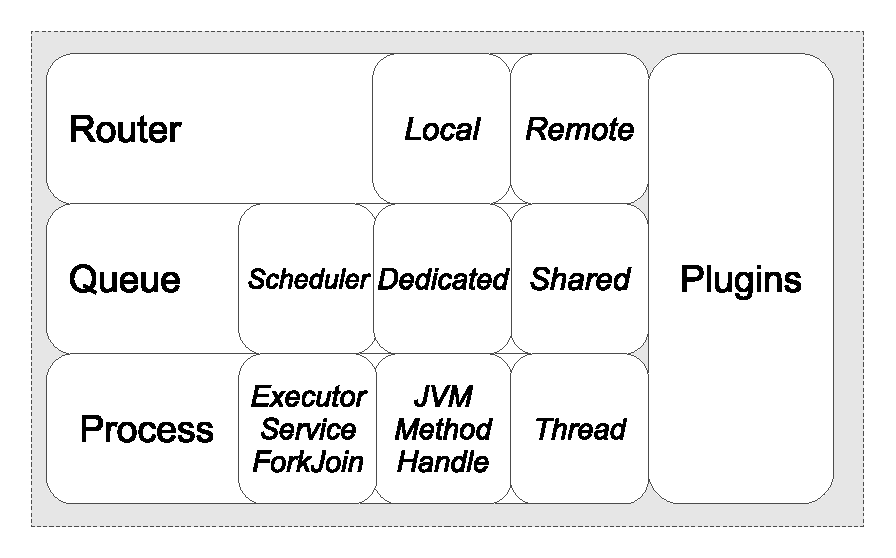
\includegraphics[scale=.6]{figs/abs-api-java8-2}  
\end{center}
\caption{Architecture of Actor API in Java~8}
\label{ch03:fig:actors:arch}
\end{figure} 

We discuss the architecture from bottom layer to top.
The implementation of actor API preserves a faithful mapping of message processing in ABS modeling language.
An actor is an active object in the sense that it controls how the next message is executed and may release any resources to allow for co-operative scheduling.
Thus, the implementation is required to optimally utilize JVM threads.
Clearly, allocating a dedicated thread to each message or actor is not scalable.
Therefore, actors need to \emph{share} threads for message execution and yet be in full control of resources when required.
The implementation fundamentally separates \emph{invocation} from \emph{execution}.
An asynchronous message is a reference to a method invocation until it starts its execution.
This allows to minimize the allocation of threads to the messages and facilitates sharing threads for executing messages.
Java concurrent API~\cite{jsr166} provides different ways to deploy this separation of invocation from execution.
We take advantage of Java Method Handles~\cite{jsr292:invokedyn} to encapsulate invocations.
Further we utilize different forms of \jtt{ExecutorService} and \jtt{ForkJoinPool} to deploy concurrent invocations of messages in different actors.

In the next layer, the actor API allows for different implementations of a queue for an actor.
A dedicated queue for each actor simplifies the process of queuing messages for execution but consumes more resources.
However, a  shared queue for a set of actors allows for memory and storage optimization.
This latter approach of deployment, first, provides a way to utilize the computing power of multi-core; 
for instance, it allows to use work-stealing to maximize the usage of thread pools.
Second, it enables  application-level scheduling of messages.
The different implementations cater for a variety of plugins, like
one that releases computation as long as there is no item
in the queue and becomes active as soon as an item is placed into the queue; e.g. \jtt{java.util.concurrent.BlockingQueue}.
Further, different plugins can be injected to allow for scheduling of messages extended with deadlines and priorities
~\cite{Nobakht:sched}.


%Each layer can be \emph{distributed} independently of another layer in a transparent way.
%  For instance, not only the routing layer can provide distribution, the queue layer of the architecture may also be remote to take advantage of cluster storages for actor messages. 
%
%
%
%
%
%
%The process of sending an asynchronous message leads to the following steps according to the actor model in ABS at the level of implementation.
%
%
%A message has a receiver actor that needs to be identified. 
%The receiver in essence has no location limitation and as such can be local or remote.
%Thus, the actor API should manage a way to \emph{route} the message to the receiver.
%The routing layer of actor API forms the foundation for the support of distribution and location transparency~\cite{KarmaniSA09} of actors.
%From the perspective of the sender of a message, the location of the receiver is hidden and only referred by a name or an address.
%It is the responsibility of the routing layer to find the appropriate receiver actor for the message.
%As a result of routing a message, the queue in which the message should be placed into is identified.

%An actor owns a queue of messages.


% When a message is sent to an actor, an \emph{envelope} is created.
% The envelope encapsulates the sender, the receiver and the method invocation of the receiver with its actual parameters.
% An envelope is \emph{routed} to its receiver; there may exist different implementations of routers such as local or remote.
% Routing an envelopes consists of discovering the appropriate \emph{inbox} to which the envelope is posted.
% When an envelope is received in an inbox, it is delegated to an \emph{opener}.
% Note that each actor is ``related'' to an inbox;
% such relation can be \emph{own}ing individually or \emph{shar}ing an inbox with other actors.
% Openning an envelope is left as an implementation detail.
% For instance, a direct simple implementation is to \emph{synchronously} open and process the envelope.
% In an asynchronous implementation, openning an envelope actually \emph{queues} it to be executed. 
% A queue of envelopes may take advantage of different JVM execution services; e.g. direct usage of \jtt{Thread}s or utilizing different types of concurrent executor services.

%The API architecture described in the above has certain properties:
%\begin{itemize}
%  \item From the perspective of the user of the API, an actor is abstraction that facilitates sending asynchronous messages and working with future values according to the actor model. Any extension or custom implementation should guarantee the same semantics of asynchronous message passing.
%  \item Each layer of the actor API is \emph{pluggable}; i.e. specific implementations can be injected into the actor API context using standard Java service loading mechanisms.
%  \item Each layer can be \emph{distributed} independently of another layer in a transparent way.
%  For instance, not only the routing layer can provide distribution, the queue layer of the architecture may also be remote to take advantage of cluster storages for actor messages. 
%  \item The \emph{invocation} is separated from \emph{execution}. 
%  An asynchronous message encapsulates and carries a method invocation; however, its execution and the properties of its execution such as priority in terms of time or order is left to a different layer. 
%  Such separation of concerns maximizes the concurrency level and utilization of computing resources in a lock-free style.
%\end{itemize}

% We discuss the distribution of actors in this architecture in the next section.
% The implementation is available at \surl{https://github.com/CrispOSS/abs-api}.
% 
% \section{Distribution of Actors}
% \label{ch03:sec:distributtion}

We discuss next the distribution of actors in this architecture.
In the architecture presented  in Figure~\ref{ch03:fig:actors:arch}, each layer can be \emph{distributed} independently of another layer in a transparent way.
Not only the routing layer can provide distribution, the queue layer of the architecture may also be remote to take advantage of cluster storage for actor messages. 
A remote routing layer can provide access to actors transparently through standard naming or addresses.
% The implementation of remote actors is left as an the extension or plugin that is injected into the system.
% For instance, an extension may choose to provide remote actor access through HTTP layer; however, another may opt for a network layer implementation.
We exploit the main properties of actor model~\cite{agha97,Agha90} to distribute actors based on our implementation.
From a distributed perspective, the following are the main requirements for  distributing actors:
\begin{description}
\item[Reference Location Transparency] 
Actors communicate to one another using references. 
In an actor model, there is no in-memory object reference; however, every actor reference denotes a location by means of which the actor is accessible.
The reference location may be local to the calling actor or remote.
The reference location is \emph{physically} transparent for the calling actor.
\item[Communication Transparency]
A message $m$ from actor $A$ to actor $B$ may possibly lead to transferring $m$ over a network such that $B$ can process the message.
Thus, an actor model that supports distribution must provide a layer of remote communication among its actors that is transparent, i.e., 
when actor $A$ sends message $m$, the message is transparently transferred over the network to reach actor $B$.
For instance, actors existing in an HTTP container that transparently allows such communication.
Further, the API implementation is required to provide a mechanism for serialization of messages.
By default, every object in JVM cannot be assumed to be an instance of \jtt{java.io.Serializable}.
However, the API may enforce  that any remote actor should have the required actor classes in its JVM during runtime which
allows the use of the JVM's general object serialization
\footnote{Java Object Serialization Specification: \surl{http://docs.oracle.com/javase/8/docs/platform/serialization/spec/serialTOC.html}}
to send messages to remote actors and receive their responses.
Additionally, we model asynchronous messages with lambda expressions for which Java~8 supports serialization by specification
\footnote{Serialized Lambdas: \surl{http://docs.oracle.com/javase/8/docs/api/java/lang/invoke/SerializedLambda.html}}.
\item[Actor Provisioning]
During a life time of an actor, it may need to create new actors.
Creating actors in a local memory setting is straightforward. 
However, the local setting \emph{does} have a capacity of number of actors it can hold.
When an actor creates a new one, the new actor may actually be initialized in a remote resource.
When the resource is not available, it should be first provisioned.
However, this resource provisioning should be transparent to the actor and only the eventual result (the newly created actor) is visible.
\end{description}

We extend the ABS API to ABS Remote API\footnote{The implementation is available at \surl{https://github.com/CrispOSS/abs-api-remote}.} 
that provides the above properties for  actors in a seamless way.
A complete example of using the remote API has been developed\footnote{An example of ABS Remote API is available at \surl{https://github.com/CrispOSS/abs-api-remote-sample}.}. 
Expanding our ping-pong example in this paper, Listing~\ref{ch03:lst:ping:remote} and \ref{ch03:lst:pong:remote} present how a remote server of actors is created for the ping and pong actors.
In the following listings, \jtt{java.util.Properties} is used provide input parameters of the actor server;
namely, the address and the port that the actor server responds to.

\begin{center}
\begin{minipage}[t]{0.48\textwidth}
\begin{lstlisting}[caption=Remote ping actor main,label=ch03:lst:ping:remote]
Properties p =  new Properties();
p.put("host", "localhost");
p.put("port", "7777");
ActorServer s = new ActorServer(p);
IPong pong = 
 s.newRemote("abs://pong@http://localhost:8888",
  IPong.class);
Ping ping = new Ping(pong);
ping.send(
  () -> ping.ping("")
);
\end{lstlisting}
\end{minipage}
\hfill
\begin{minipage}[t]{0.48\textwidth}
\begin{lstlisting}[caption=Remote pong actor main,label=ch03:lst:pong:remote]
Properties p = new Properties();
p.put("host", "localhost");
p.put("port", "8888");
ActorServer s = new ActorServer(p);
Pong pong = new Pong();
\end{lstlisting}
\end{minipage}
\end{center}

In Listing~\ref{ch03:lst:ping:remote}, a remote reference to a pong actor is created that exposes the \jtt{IPong} interface.
This interface is proxied
\footnote{Java Proxy: \surl{http://docs.oracle.com/javase/8/docs/api/java/lang/reflect/Proxy.html}} by the implementation 
to handle the remote communication with the actual pong actor in the other actor server.
This mechanism hides the communication details from the ping actor and as such allows the ping actor to use 
the same API to send a message to the pong actor (without even  knowing that the pong actor is actually remote).
When an actor is initialized in a distributed setting it transparently identifies its actor server and registers with it.
The above two listings are aligned with the similar main program presented in Listing~\ref{ch03:lst:main:api} that presents the same in a local setting.
The above two listings run in separate JVM instances and therefore do not share any objects.
In each JVM instance, it is required that both interfaces \jtt{IPing} and \jtt{IPong} are visible to the classpath; however, 
the ping actor server only needs to see \jtt{Ping} class in its classpath and similarly the pong actor server only needs 
to see \jtt{Pong} class in its classpath.

\section{Experiments}
\label{ch03:sec:experiments}

In this section, we explain how a series of benchmarks were directed to evaluate the performance and functionality of actor API in Java 8.
For this benchmark, we use a simple Java application that uses the ``Ping-Pong'' actor example discussed previously. 
An application consists of one instance of \jtt{Ping} actor and one instance of \jtt{Pong} actor. 
The application sends a \jtt{ping} message to the ping actor and waits for the result.
The ping message depends on a \jtt{pong} message to the pong actor.
When the result from the pong actor is ready, the ping actor completes the message;
this completes a round trip of a message in the application.
To be able to make comparison of how actor API in Java 8 performs, the example is also implemented using Akka~\cite{akka} library. 
The same set of benchmarks are performed in isolation for both of the applications.
To perform the benchmarks, we use JMH~\cite{jmh} that is a Java microbenchmarking harness developed by OpenJDK community and used to perform benchmarks for the Java language itself.

\begin{figure}[t]
\begin{center}
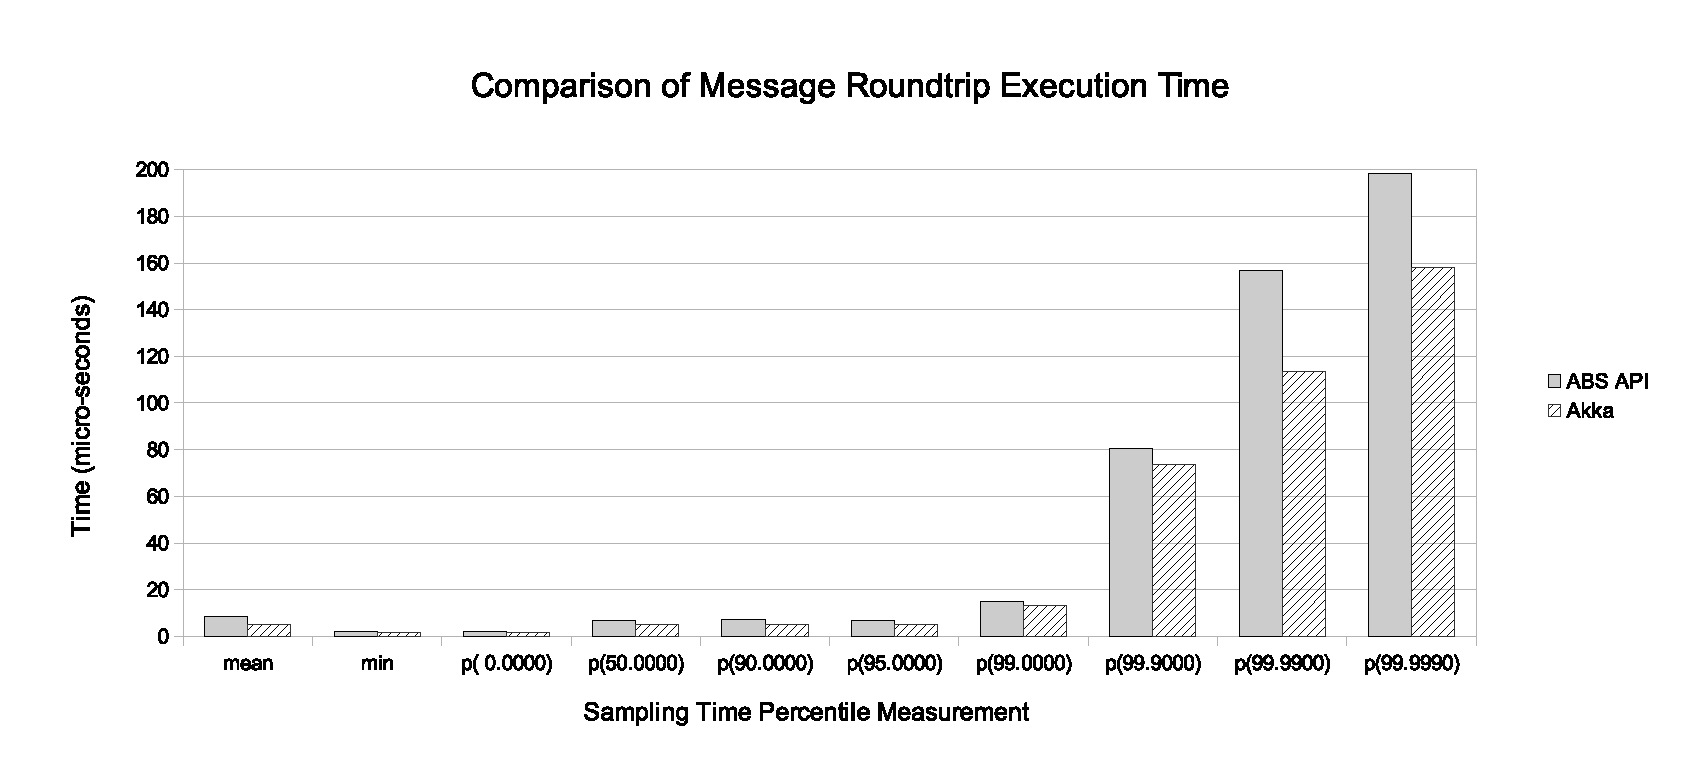
\includegraphics[scale=.45]{figs/benchmarks}  
\end{center}
\caption[Benchmarking comparison of ABS API and Akka]{
Benchmark results of comparing sampling time of message round trips in ABS API and Akka.
An example reading of above results is that the time shows for $p(90.0000)$ reads as ``message round trips were completed under $10{\mu}s$ for $90\%$ of the sent messages''.
The first two columns show the ``minimum'' and ``mean'' message round trip times in both implementations.
}
\label{ch03:fig:benchmarks}
\end{figure} 

The benchmark is performed on the round trip of a message in the application. 
The benchmark starts with a warm-up phase followed by the running phase.
The benchmark composes of a number of iterations in each phase and specific time period for each iteration specified for each phase.
Every iteration of the benchmark triggers a new message in the application and waits for the result.
The measurement used is \emph{sampling time} of the round trip of a message.
A specific number of samples are collected. 
Based on the samples in different phases, different \emph{percentile} measurements are summarized.
An example percentile measurement $p(99.9900) = 10 \; {\mu}s$ is read as $99.9900\%$ of messages in the benchmark took 10 micro-seconds to complete. 

Each benchmark starts with 500 iterations of warm-up with each iteration for 1 micro-second.
Each benchmark runs for 5000 iterations with each iteration for 50 micro-seconds.
In each iteration, a maximum number of 50K samples are collected.
Each benchmark is executed in an isolated JVM environment with Java 8 version b127.
Each benchmark is executed on a hardware with 8 cores of CPU and a maximum memory of 8GB for JVM.

The results are presented in Figure \ref{ch03:fig:benchmarks}.
The performance difference observed in the measurements can be explained as follows.
An actor in Akka is expected to expose a certain behavior as discussed in Section \ref{ch03:sec:example} (i.e. \jtt{onReceive}).
This means that every message leads to an eventual invocation of this method inside actor.
However, in case of an actor in Java~8, there is a need to make a look-up for the actual method to be executed with expected arguments. 
This means that for every method, although in the presence of caching, there is a need to find the proper method that is expected to be invoked. 
A constant overhead for the method look-up  in order to adhere to the object-oriented principles is naturally to be expected.
Thus, this is the minimal performance cost that the actor API in Java~8 pays to support  programming to interfaces.

\section{Conclusion}
\label{ch03:sec:conclusion}

In this paper, we discussed an implementation of the actor-based ABS modeling language
in Java~8 which supports  the basic object-oriented mechanisms
and principles of method look-up and programming to interfaces.
In the full version of this paper we have developed an operational semantics of Java~8 features including lambda expressions 
and have proved formally the correctness of the embedding in terms of a bisimulation relation.

The underlying modeling language has an executable semantics
and supports a variety of formal analysis techniques, including
deadlock and schedulability analysis \cite{GiachinoGLLW13,JaghooriBCS09}.
Further it supports a formal 
behavioral specification of interfaces \cite{hahnlehjlssw11}, to be used as contracts.




We intend to expand this work in different ways.
We aim to automatically \emph{generate} ABS models from Java code which follows the ABS
design methodology.
Model extraction allows industry level applications be abstracted into models and 
analyzed for different goals such as deadlock analysis and concurrency optimization.
This approach of model extraction we believe will greatly enhance industrial uptake of formal methods.
We aim to further extend the implementation of API to support different features especially regarding distribution of actors especially in the queue layer, and scheduling of messages using application-level policies or real-time properties of a concurrent system.
Furthermore, the current implementation of ABS API in a distributed setting allows for instantiation of remote actors. 
We intend to use the implementation to model ABS deployment components~\cite{johnsen2012modeling} and simulate a distributed environment.

% Bibliography
% \bibliographystyle{plain}
% \bibliography{refs}
